\chapter{Gait Watch and Force Plate signals processing}
\label{ch:GWandFP}

\section{Introduction and chapter's structure}

\section{Data gathering Protocol}
Prior to start of data gathering, it’s necessary to set up the protocol for procedure that patients have to carry out while the data are recorded. The establishing this procedure is very important so that the synchronisation works properly because we have to identify a clear movement in both signals to match one signal with the other at the same time.
In addition, the realised movements must be representatives to obtain conclusive data which help us to extract characteristics for the purpose of identify differences between patients and control subjects subsequently.

The steps followed by the patients are detailed hereafter:

1.	Subject stands in front of the Force Plate.

2.	Gait watch record starts for data gathering.

3.	Force plate record starts for data gathering.

4.	Subject makes a step onto the platform.

5.	Subject stands on the platform a variable time between 2 and 10 seconds.

6.	Subject makes some step  forward and turns left to stand in front of the platform again.

This procedure is repeated ten times by each subject in order to characterise better the movement made.
It’s important to clarify that the GaitWatch recording contains all these ten episodes ( in other cases more) and the platform recording only contains one episode each. So, this is a fact that we have to consider to do the synchronisation.

\section{Synchronisation}
\subsection{Introduction and chapter's structure}
One of the most important aspects whether you have data acquired from multiples devices or channels is the synchronisation. If these data are not appropriately correlated or synchronised, the analysis and conclusions from your use will be erroneous. Also, it’s very important doing all automatically when you have a data on a broad scale.
Therefore, the following sections explain how the information has been obtained and processed automatically, as well as what features have been calculated to characterise the movements of the patients and to carry out the synchronisation between the Force Plate signals and GaitWatch signals. This content is superficially depicted in figure XX.

\begin{figure}[H]
	\centering
	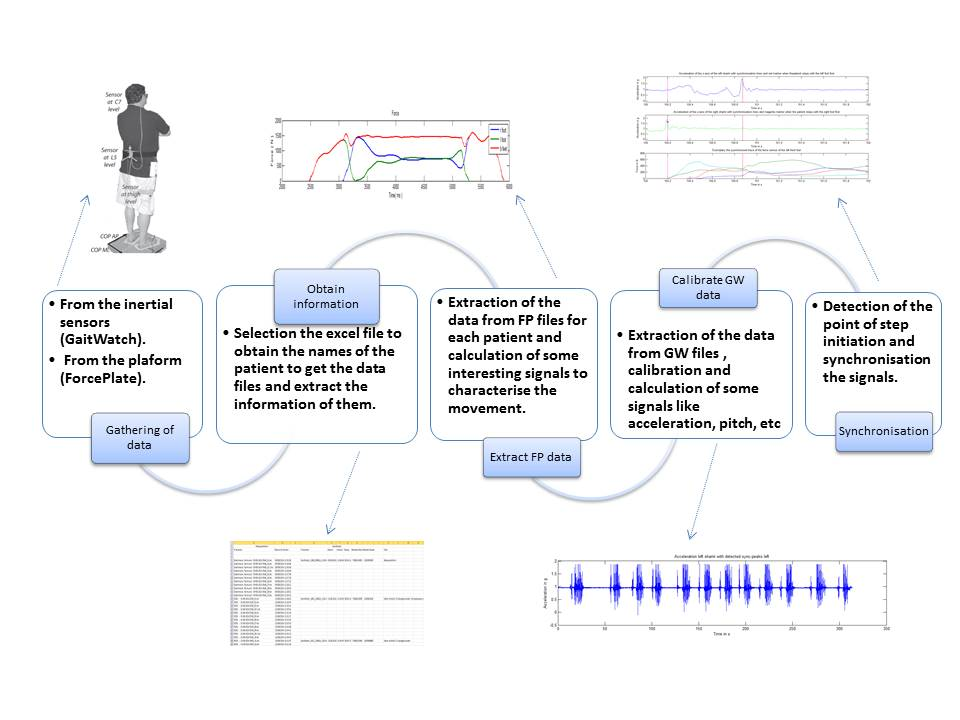
\epsfig{file=imagenes/diagramSynchronisation, width=8cm}
	\caption{Diagram of the Synchronisation's progress.}
	\label{fig:arte1}
\end{figure}

\subsection{Design of developed code  in Matlab}
\subsubsection{Selection, reading and obtaining of information from the excel file}
\subsubsection{Extraction of the forceplate data}
\subsubsection{Calibration of the GaitWatch data}
\subsubsection{Synchronisation}	
\subsection{Results discurssion}


\section{APA analysis}

